\chapter{Results}\label{results}

The goal of this thesis is to determine whether using data from political party manifestos can enhance party stance prediction. To do this, a model that examines user-generated statements and predicts if the parties will agree with them is built. To add more context, the model is also fed relevant passages from party manifestos.

The thesis discusses several semantic search techniques for locating relevant passages in the manifestos and evaluates various input patterns to determine the most effective means of conveying this additional information to the model. Additionally, it compares how ELECTRA \citep{clark2020electra} and BERT \citep{devlin2018bert} perform when given these various inputs.

For each model, 49 inputs were evaluated, including one without any added context, which served as a baseline with no semantic search. The models' performance was evaluated by calculating the accuracy on the test data.

\section{ELECTRA}

\begin{figure}[h]
\centering
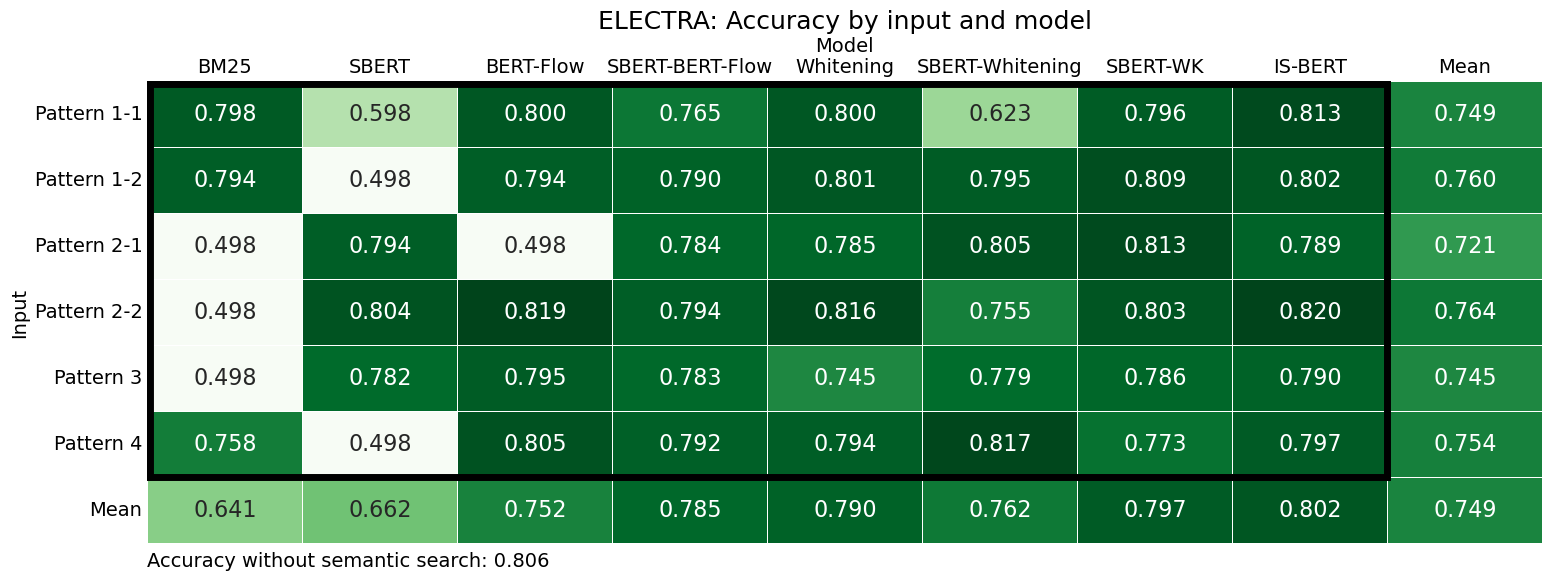
\includegraphics[width = 1\linewidth]{figures/electra_accuracy.png}
\caption{The accuracy calculated on the test data for all models with ELECTRA as the base model}
\label{fig:electra_accuracy}
\end{figure}

The performance of ELECTRA was evaluated using various combinations of semantic search techniques and input patterns, and the results are presented in Figure \ref{fig:electra_accuracy}. It displays the accuracy scores of the ELECTRA models with and without semantic search. The accuracy without semantic search is 0.806 (displayed below the table), which serves as a baseline for comparing the performance of models that utilize semantic search techniques to provide additional context. Interestingly, only seven out of the 48 context-based models outperformed the baseline model without semantic search. Six models only ever predict agreement (accuracy of 0.498) regardless of the query. This issue was mostly observed in the BM25 models, with three out of the six BM25 models suffering from this problem. The average accuracy for BM25 was the lowest (0.641), while SBERT models performed slightly better, followed by BERT-Flow, SBERT-Whitening, SBERT-BERT-Flow, Whitening, and SBERT-WK. On the other hand, IS-BERT was the most effective semantic search technique overall. The two Whitening models (SBERT-Whitening and Whitening) and the two BERT-Flow models (SBERT-BERT-Flow and BERT-Flow) don't seem to behave similarly to each other.

Notably, the various input patterns produced similar accuracy scores, with Pattern 2-2 performing the best and Pattern 3 performing the worst. Interestingly, the performance of the input patterns does not follow a discernible pattern. Patterns sharing similar properties do not show a consistent performance trend, Patterns 1-1 and 1-2 or 2-1 and 2-2 do not exhibit similar behaviors.

\section{BERT}

\begin{figure}[h]
\centering
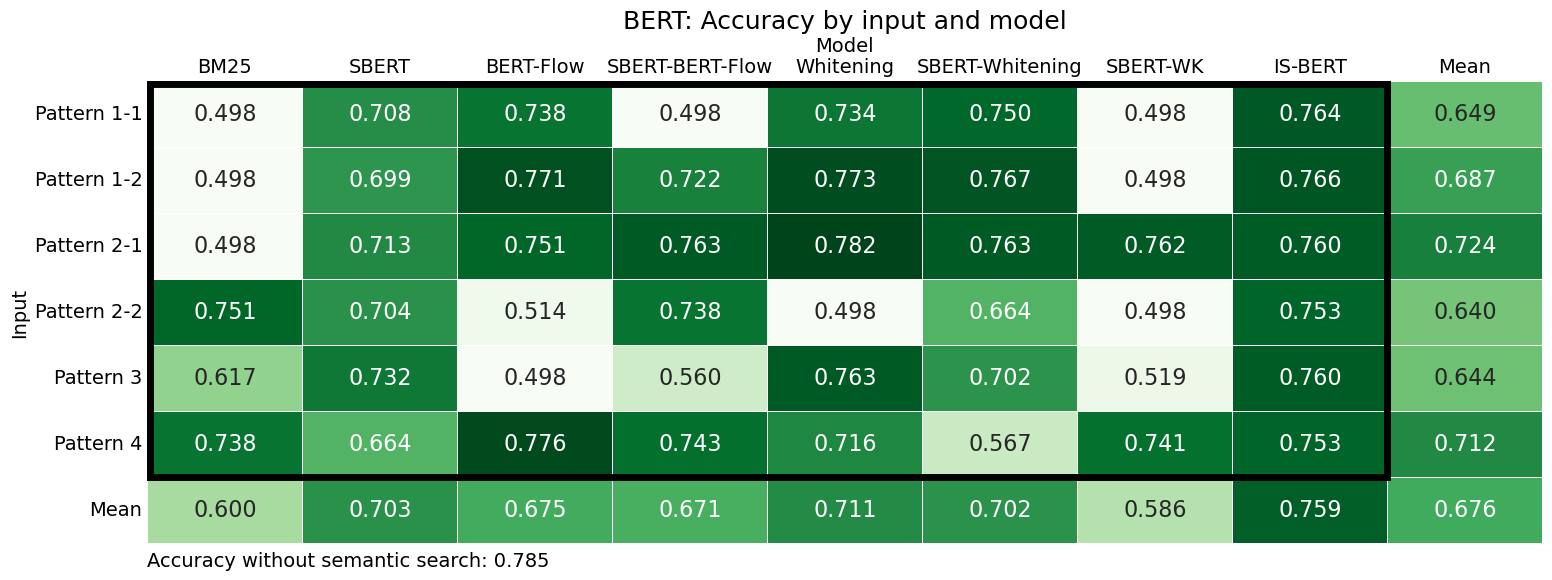
\includegraphics[width = 1\linewidth]{figures/bert_accuracy.png}
\caption{The accuracy calculated on the test data for all models with BERT as the base model}
\label{fig:bert_accuracy}
\end{figure}

Figure \ref{fig:bert_accuracy} presents the results of all models that used BERT as the base model. Overall, the models that incorporated semantic search performed worse than the baseline without semantic search (0.786), with a notable number of models that always predict agreement regardless of the query. Among the semantic search techniques, IS-BERT outperforms the others with a mean accuracy of 0.759, followed by Whitening, SBERT, and SBERT-Whitening. While BERT-Flow and SBERT-BERT-Flow perform better than the baseline BM25, SBERT-WK performs even worse. Again, there seems to be no correlation between how the two Whitening models and the two BERT-Flow models behave.

The two best-performing input patterns are Pattern 2-1 and Pattern 4, while Pattern 3 and Pattern 2-2 perform the worst in terms of accuracy. Once more, there is no discernible pattern in how the input patterns perform.

\section{Main Results}

The results of both the ELECTRA and BERT experiments indicate that incorporating additional context through semantic search techniques does not necessarily improve the performance of the models. In fact, the accuracy of most models that used semantic search were worse than the baseline model without it. However, IS-BERT showed promising results and performed consistently well across all patterns, indicating its effectiveness in this task. On the other hand, models that used BM25 as the semantic search technique performed poorly. The different input patterns did not show a big difference in performance, with only slight variations in accuracy. A considerable number of models showed poor performance by only predicting agreement. Additionally, the best-performing model only had a marginal improvement over the baseline. The experiments revealed that, on average, the ELECTRA models outperformed the BERT models, supporting the findings of \citet{witte_2022}.

\section{Further Experiments}

\begin{figure}[h]
\centering
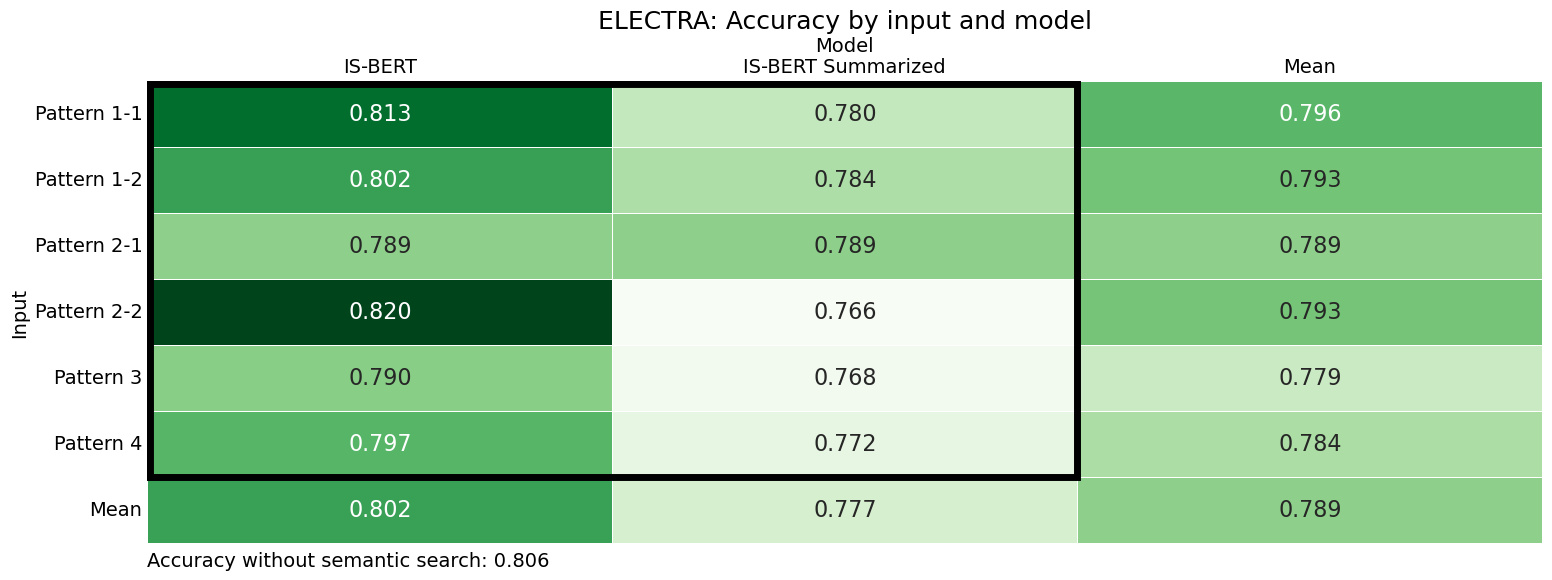
\includegraphics[width = 1\linewidth]{figures/electra_summary_accuracy.png}
\caption{The accuracy calculated on the test data for the IS-BERT and IS-BERT Summarized models (with ELECTRA as the base model)}
\label{fig:electra_summary_accuracy}
\end{figure}

The findings of the summarization experiment discussed in Chapter \ref{exp_further} are shown in Figure \ref{fig:electra_summary_accuracy}. As can be seen, none of the models that make use of the summarized context perform better than the baseline of no context. The worst IS-BERT model without summarization performs equally well as the best result with summarization (accuracy of 0.789). All models perform better without summarization, with the exception of pattern 2-1 (which performs the same).
